\documentclass[../HAFiscal]{subfiles}
\begin{document}

\FloatBarrier
\section{Robustness}
\label{sec:robustness}

In this section we analyze how sensitive our results are to some of the parameters in the model. In particular, we focus on parameters that heavily influence consumers' incentives to save. These parameters are the interest rate that affects the returns on saving, and the degree of risk aversion and the replacement rates when unemployed with or without benefits that affect the strength of a precautionary saving motive. The aim is to alter these incentives while maintaining the requirement that the distributions of liquid wealth in each education group matches the distributions in the data. Hence, in each case, we reestimate the distributions of discount factors in each education group (and, if necessary, the degree of `splurge' spending in consumption). The aim is thus to compute new results for a model with different parameters that also fits data on the distribution of liquid wealth. 

\subsection{Changing the interest rate}
\label{sec:robust_R} 
In our baseline calibration, the interest rate is set to $1$ percent per quarter. Here we consider the impact on our results of increasing or decreasing this value. Changes to the U.S. interest rate do not affect the estimation of the splurge-parameter $\varsigma$. However, before we can calculate updated results for a different interest rate, the distribution of discount factors within each education group must be reestimated for the model to continue to match the liquid wealth distributions. 

\subsubsection{Discount factor distributions with different interest rates}
\label{sec:robust_R_estim}

Table~\ref{tab:robustness_R} shows the values we obtain for the discount factor distributions when we change the quarterly interest rate by either decreasing it to $0.5$ percent or increasing it to $1.5$ percent. In both cases, the estimation can match the median liquid wealth to permanent income ratios for each education group reported in Panel~B of Table~\ref{tab:estimBetas} exactly. 

\begin{table}[t]
\begin{center}
	\begin{tabular}{lc|cccccc} 
		\toprule
		& & \multicolumn{2}{c}{Dropout} & \multicolumn{2}{c}{Highschool} & \multicolumn{2}{c}{College} \\ \midrule 
		& Splurge & $\beta$ & $\nabla$ & $\beta$ & $\nabla$ & $\beta$ & $\nabla$ \\ \midrule 
		$R = 1.005$ & 0.307 & 0.701 & 0.520 & 0.909 & 0.099 & 0.983 & 0.014 \\
		$R = 1.01$ (baseline) & 0.307 & 0.694 & 0.542 & 0.904 & 0.099 & 0.978 & 0.015 \\ 
		$R = 1.015$ & 0.307 & 0.691 & 0.542 & 0.899 & 0.099 & 0.973 & 0.016 
		\\ \bottomrule 
	\end{tabular}
\end{center}
\caption{Estimates of the Splurge and $(\beta,\nabla)$ for each education group for different values of the interest rate $R$.}
\label{tab:robustness_R}
\end{table}

The first row of Table~\ref{tab:robustness_R} shows the estimated $\beta_e$ and $\nabla_e$ for the lower interest rate of $0.5$ percent per quarter. With a lower interest rate and an unchanged discount factor distribution, consumers would tend to substitute away from saving and towards current consumption. They would therefore accumulate less wealth leading to a lower median liquid wealth to permanent income ratio. In all education groups we therefore see that the estimated discount factor distributions are centered around higher values of $\beta$ to ensure that the model still matches the median liquid wealth to permanent income ratio in the data. An increase in patience cancels out the effect of the lower interest rate on median saving. Similarly, in the third row, we see the opposite effect when the interest rate is increased to $1.5$ percent.  

Figure~\ref{fig:LorenzPts_robustness_R} in Appendix~\ref{app:DF_R} shows that the reestimated model also matches the liquid wealth distributions for each of these values of the interest rate. From Table~\ref{tab:robustness_R} we see that the values of $\nabla_e$ for the three education groups do not need to change much for this to be the case. 

\subsubsection{Results for different interest rates}
\label{sec:robust_R_results}

[Ivan: fill out these results]


\subsection{Changing risk aversion} 
\label{sec:robust_gamma} 

In our baseline calibration consumers have a risk aversion of $\gamma=2$ which is quite common in macroeconomic models. Here we investigate how alternative values of $\gamma$ would influence our results. Again, we reestimate the distribution of discount factors within each education group, but in this case we also reestimate the degree of `splurge' spending in consumption. 

\subsubsection{Discount factor distributions with different risk aversion}
\label{sec:robust_gamma_estim}

Table~\ref{tab:robustness_gamma} displays the values we obtain for the splurge and the discount factor distributions when we change $\gamma$ to $1$ and $3$. The table shows that the splurge is not very sensitive to the degree of risk aversion. The splurge controls the degree of spending that consumers do before considering the trade-off involved in optimally allocating spending over time and across different future states of the world. Risk aversion affects that trade-off, but does not have a big influence on a parameter that controls spending that is independent of that problem. 

\begin{table}[t]
\begin{center}
\begin{tabular}{lc|cccccc} 
	\toprule
	& & \multicolumn{2}{c}{Dropout} & \multicolumn{2}{c}{Highschool} & \multicolumn{2}{c}{College} \\ \midrule 
	& Splurge & $\beta$ & $\nabla$ & $\beta$ & $\nabla$ & $\beta$ & $\nabla$ \\ \midrule 
	$\gamma = 1.0$ & 0.314 & 0.671 & 0.464 & 0.948 & 0.121 & 0.992 & 0.017 \\ 
	$\gamma = 2.0$ (baseline) & 0.307 & 0.694 & 0.542 & 0.904 & 0.099 & 0.978 & 0.015 \\
	$\gamma = 3.0$ & 0.304 & 0.565 & 0.749 & 0.843 & 0.163 & 0.964 & 0.027 
	\\ \bottomrule 
\end{tabular}
\end{center}
\caption{Estimates of the Splurge and $(\beta,\nabla)$ for each education group for different values of risk aversion, $\gamma$. $*$ indicates a value that is fixed in the estimation --- this is necessary in some cases to prevent the estimation procedure from trying negative values for the discount factor of some type.}
\label{tab:robustness_gamma}
\end{table}

Rows two and three of Table~\ref{tab:robustness_gamma} show results when we increase risk aversion from $\gamma=2.0$ to $\gamma=3.0$. Increasing risk aversion for all types within an education group makes the precautionary saving motive stronger for all consumers in that group. Ceteris paribus these consumers would then increase the amount of liquid wealth they accumulate, and the median liquid wealth to permanent income ratio for the education group would increase. For all the education groups the discount factor distributions are therefore centered around lower values of $\beta$ when risk aversion is increased to $3.0$. As for the increase in the interest rate in section~\ref{sec:robust_R_estim}, the decrease in patience counteracts the stronger incentive to save from the higher risk aversion. The reductions in $\beta$ when increasing risk aversion from $2.0$ to $3.0$ are much larger than when increasing the interest rate from $1$ to $1.5$ percent, however. 

The effects on $\nabla$ and the concentration of the liquid wealth distribution may be less intuitive. However, if the only changes were to increase risk aversion and to decrease $\beta$ while keeping $\nabla$ fixed at the value for $\gamma=2.0$, then the result would be a liquid wealth distribution that was much less concentrated than in the data. If all consumers in an education group are less patient, the reduction in saving is larger for the wealthier consumers. Thus, to maintain the concentrated wealth distribution $\nabla$ increases substantially. The results are distributions of discount factors within each education group that are centered around lower values, but that are much more dispersed. The effect is that the discount factor for the most patient type within each education group is not changed very much, but the lowest discount factor is much lower than when $\gamma=2.0$, and the liquid wealth distributions remain as concentrated as they are in the data also in the model where risk aversion is increased.\footnote{Note that as in the baseline case, the discount factor for the most patient type in the Dropout group is constrained by the GIC. When $\gamma=3.0$ a constraint is also binding for the least patient type. The large value of $\nabla$ relative to $\beta$ would imply a negative discount factor, and to prevent this we constrain the lowest discount factor to be $0.01$.}

When we decrease risk aversion to $\gamma=1.0$ we run into problems when estimating the discount factor distribution, however. Row~1 of Table~\ref{tab:robustness_R} shows estimated parameters that give the model the best fit for the median liquid wealth permanent income ratios and the liquid wealth distributions for each education group. The results for the $\beta$ parameters reverse the intuition that we discussed for the case $\gamma=3.0$. In this case, reducing risk aversion and the strength of the precautionary saving motive is counteracted by centering the discount factor distributions around higher values. To obtain the same amount of saving on average, consumers need to be more patient if they are less risk averse.  

\begin{table}{th}
\begin{center}
\begin{tabular}{lccc}
	\multicolumn{4}{l}{Median liquid wealth to permanent income ratios} \\ \midrule
	& Dropout & Highschool & College \\ \midrule
	Median LW/PI (data) & 4.64 & 30.2 & 112.8 \\ 
	Median LW/PI (model, $\gamma = 1.0$) & 0.00 & 30.1 & 112.8 \\	
	Median LW/PI (model, $\gamma = 2.0$) & 4.64 & 30.2 & 112.8 \\
	Median LW/PI (model, $\gamma = 3.0$) & 4.64 & 30.2 & 112.8 \\ \bottomrule
\end{tabular}
\end{center}	
\end{table}

Table~\ref{tab:robustness_gamma} shows that for $\gamma=1.0$, while the model can match the median liquid wealth to permanent income ratios for the Highschool and College groups, it does not do that for the Dropout group. Figure~\ref{fig:LorenzPts_robustness_CRRA} on the other hand shows the opposite results for matching the liquid wealth distribution within each education group: The model matches the distribution for the Dropout group, but not for the Highschool and College groups. 

\begin{figure}[th]
	\begin{center}
		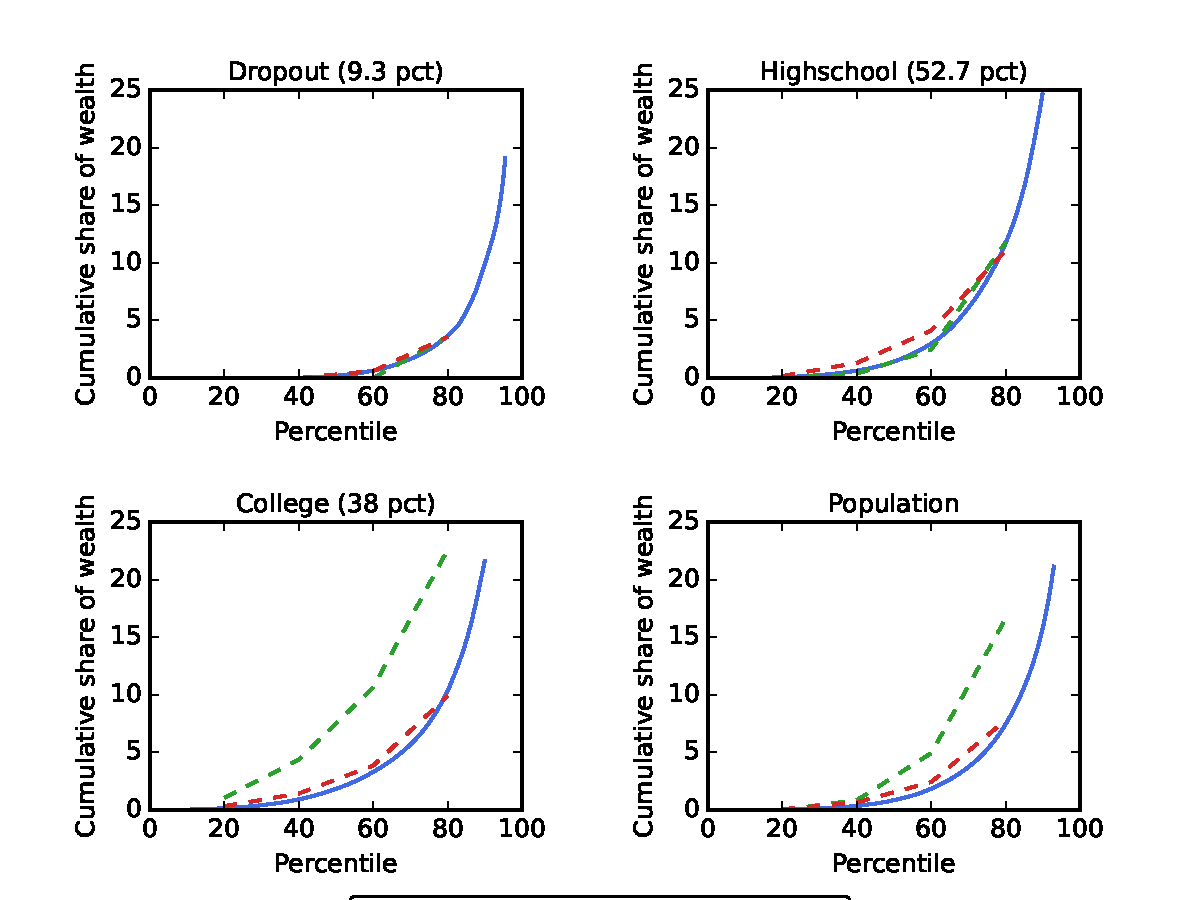
\includegraphics[width=.9\textwidth]{../Figures/LorenzPoints_robustness_CRRA.pdf}
		\caption{Distributions of liquid wealth within each educational group and for the whole population from the 2004 Survey of Consumer Finance and from the estimated model for different values of risk aversion, $\gamma$.}
		\label{fig:LorenzPts_robustness_CRRA}
	\end{center}
\end{figure}

The issue is that with a lower value of risk aversion and a weaker precautionary saving motive, the model requires consumers who are much more patient to obtain the same level and distribution of saving as in the baseline case with $\gamma=2.0$. In each education group the most patient types are then constrained by the Growth Impatience Condition. When several types are constrained, then varying the estimated parameter values further may not improve on the fit of the model. Hence, the estimation terminates when hitting only one of the two targets. 

The strength of the precautionary saving motive is not only determined by risk aversion, however. The risks that households face also drive the strength of this motive for saving, and in our model, a key risk is unemployment risk. Therefore, the replacement rates that households face when they are unemployed with or without benefits play an important role. In Section~\ref{sec:robust_benefits} we consider an alternative calibration of these values. 

\subsubsection{Results with different risk aversion}
\label{sec:robust_gamma_results}

[Ivan: fill out these results]


\subsection{Changing benefits} 
\label{sec:robust_benefits} 

In our baseline calibration we follow \cite{rothstein2017scraping} and calibrat the replacement rates to $\rho_b=0.7$ with unemployment benefits and $\rho_{nb}=0.5$ without benefits. Here we consider replacement rates that are considerably less generous and more in line with values used in the previous macro literature with unemployment in models with heterogeneous agents. The alternative values we consider are a replacement rate of $\rho_{b}=0.3$ when unemployed with benefits as in \cite{carroll2020modeling}, and a replacement rate of $\rho_{nb}=0.15$ when unemployed without benefits. This latter value is the same as the replacement rate used in \cite{den2010computational}.\footnote{In \cite{den2010computational}, there is only one unemployment state and, hence, no sense in which benefits expire after a while. Therefore, this replacement rate applies for long-term unemployed as it does in our model, but in this paper there is also an intermediate state in which benefits are higher until they expire.} With these replacement rates, being unemployed is more serious for consumers than in our baseline calibration and the precautionary saving motive is stronger. 

\subsubsection{Discount factor distributions with different benefits}
\label{sec:robust_benefits_estim}

Table~\ref{tab:robustness_benefits} shows that when benefits are less generous and the precautionary motive is stronger, then the estimated discount factor distributions are centered on lower values of $\beta$ and the dispersion in the distributions increase as $\nabla$ is considerably higher. The intuition is similar to the case when increasing risk aversion from $\gamma=2.0$ to $\gamma=3.0$ discussed in section~\ref{sec:robust_gamma_estim}: A stronger precautionary motive for saving must be counteracted by a lower average discount factor to match the same average level of saving as before. The distributions must also be more dispersed to match the same concentration of liquid wealth. In fact, the estimated discount factor distributions for the alternative calibration of the replacement rates are very similar to those reported for $\gamma=3.0$ in row~3 of Table~\ref{tab:robustness_gamma}. 

\begin{table}[t]
\begin{center}
	\begin{tabular}{llc|cccccc} 
		\toprule
		& & & \multicolumn{2}{c}{Dropout} & \multicolumn{2}{c}{Highschool} & \multicolumn{2}{c}{College} \\ \midrule 
		& & Splurge & $\beta$ & $\nabla$ & $\beta$ & $\nabla$ & $\beta$ & $\nabla$ \\ \midrule 
		Baseline & ($\rho_{b}=0.7$ and $\rho_{nb}=0.5$) & 0.307 & 0.694 & 0.542 & 0.904 & 0.099 & 0.978 & 0.015 \\ 
		Alternative & ($\rho_{b}=0.3$ and $\rho_{nb}=0.15$) & 0.307 & 0.599 & 0.687 & 0.852 & 0.159 & 0.968 & 0.028
		\\ \bottomrule 
	\end{tabular}
\end{center}
\caption{Estimates of the Splurge and $(\beta,\nabla)$ for each education group for the baseline replacements rates $\rho_{b}$ and $\rho_{nb}$ and an alternative calibration.}
\label{tab:robustness_benefits}
\end{table}


\subsubsection{Results with different benefits}
\label{sec:robust_benefits_results}

[Ivan: fill out these results]

\subsection{Summary of robustness exercises}
\label{sec:robust_summary}

\end{document}	